\documentclass[a4paper,11pt]{article}

\usepackage{times}
%\setcounter{secnumdepth}{0} % sections are not getting numbered
\usepackage[english,serbian]{babel}


\usepackage[T1]{fontenc} 
\usepackage{biblatex} % bibliography

\addbibresource{citation.bib} % file with references


\usepackage{comment}
\usepackage{amsfonts}
\usepackage{amsmath}
\usepackage{amsthm}
\usepackage{IEEEtrantools}
\usepackage{graphicx}
%\usepackage{cite}

%\usepackage{geometry}
%\usepackage{upgreek}
\usepackage[serbian]{babel}
%\usepackage{ulem}
%\usepackage{environ}
\usepackage{tikz}
\usepackage{color}
\usepackage{fancybox}

%\numberwithin{equation}{section}
\theoremstyle{definition} \newtheorem{deff}{Definicija}[section]
\theoremstyle{definition} \newtheorem{prim}[deff]{Primer}
\theoremstyle{plain} \newtheorem{teor}[deff]{Teorema}


\newcommand{\unija}[2]{#1 \cup #2}
\newcommand{\pres}[2]{#1 \cap #2}
\newcommand{\tnorm}{$t$-norm}
\newcommand{\tkonorm}{$t$-konorm}
\newcommand{\vect}[1]{\boldsymbol{\mathbf{#1}}}

\renewenvironment{proof}[1][\proofname]{{\bfseries #1.}}

\frenchspacing


\usepackage[a4paper,top=3cm,bottom=2cm,left=2cm,right=2cm,marginparwidth=1.75cm]{geometry}
%% Useful packages
\usepackage{mathrsfs}
\newsavebox\foobox
\newlength{\foodim}
\newcommand{\slantbox}[2][0]{\mbox{%
		\sbox{\foobox}{#2}%
		\foodim=#1\wd\foobox
		\hskip \wd\foobox
		\hskip -0.5\foodim
		\pdfsave
		\pdfsetmatrix{1 0 #1 1}%
		\llap{\usebox{\foobox}}%
		\pdfrestore
		\hskip 0.5\foodim
}}
\def\Laplace{\slantbox[-.45]{$\mathscr{L}$}}

%\usepackage[colorinlistoftodos]{todonotes}

\usepackage{caption}
\usepackage{subcaption}
\usepackage{changepage}
\usepackage{multirow}

\usepackage{blindtext}

\usepackage{tabularx}
\usepackage[export]{adjustbox}

\usepackage[utf8]{inputenc}
\usepackage[T1]{fontenc}
\usepackage{lmodern}
\usepackage{graphicx}
\usepackage{color}
\usepackage{listings}
\usepackage{amsmath}

%\usepackage[usenames,dvipsnames]{xcolor}
%\usepackage[colorlinks=true,linkcolor=blue]{hyperref}

\usepackage{amsfonts}
\usepackage{epstopdf}

\usepackage{float}

\usepackage[shortlabels]{enumitem}
\usepackage[yyyymmdd]{datetime}


\renewcommand{\figurename}{Slika}

\DeclareMathOperator*{\argmax}{\arg\max}
\graphicspath{{./images/}}

\usepackage{booktabs}

\usepackage{siunitx}

\usepackage{scalerel}




\sloppy

\epstopdfsetup{update} % only regenerate pdf files when eps file is newer

%%%%%%%% DOCUMENT %%%%%%%%
\setlength {\marginparwidth }{2cm}
\begin{document}
	
	%%%% Title Page
	\begin{titlepage}
		
		\newcommand{\HRule}{\rule{\linewidth}{0.5mm}} 							% horizontal line and its thickness
		\center 
		
		% University
		\textsc{\LARGE Elektrotehnički fakultet u Beogradu}\\[1cm]
		
		% Document info
		\textsc{\Large Optimalno upravljanje sistemima}\\[0.2cm]
		\textsc{\large 13M051OUS}\\[1cm] 										
		\HRule \\[0.8cm]
		{ \huge \bfseries Upravljanje dvostrukim inverznim klatnom}\\[0.7cm]								% Assignment
		%\HRule \\[2cm]
		\textsc{\large Projektni zadatak broj 2}\\[1cm]
		
		
		\large
		\vfill 
		\emph{Studenti:}\\
		Nikita Jokić 3279/2023\\[0.1cm]
		Ivona Dučić 3067/2023\\[1.5cm]		
		\emph{Mentor:}\\
		doc. dr Aleksandra Krstić\\[0.1cm]									
		{\large Avgust 2024}\\[2cm]
	\end{titlepage}
	\tableofcontents
	\newpage
	
	\section{Modeliranje sistema i analiza modela}\label{sec:mod i an}
	\subsection{Uvod} 
	
	Furuta penduluma (FP) je rotaciono klatno koje se pokreće motorom jednosmerne struje. Dva najveća zahteva u vezi sa ovim sistemom su podizanje klatna iz donjeg u gornji položaj i održavanje klatna u uspravnom, nestabilnom ravnotežnom stanju. U ovom radu razmatrane su  strategije upravljanja za nelinearni problem uspravljanja i balansiranja FP u uspravnom  položaju. Iako ovo može delovati kao akademski problem, FP je ilustrativan za širok spektar dinamičkih sistema sa stvarnim primenama. Fokusiranje na ovu problematiku integrisano je u aktuelna istraživanja u oblasti sajber-fizičkih sistema (CPSs)\footnote{Sajber-fizički sistemi (CPSs) predstavljaju integraciju računarskih elemenata sa fizičkim sistemima, stvarajući tako dinamičko i uzajamno povezano okruženje.} \cite{inicijalna}. \\ 
	
	%	Fizičari su uspešni u modelovanju fenomena u prirodi u iznenađujućem broju redova veličina. Iako se u većini slučajeva može samo težiti posmatranju, u malom, ali važnom podskupu, moguće je aktivno modifikovati ponašanje sistema. Ovo se postiže uključivanjem računarskih komponenti koje interaguju sa fizičkim sistemom, što čini osnovu istraživanja u oblasti sajber-fizičkih sistema. Teorija upravljanja se bavi izazovima u postizanju željenih performansi sistema, uključujući nestabilnost u otvorenoj sprezi, ograničenja u broju promenljivih koje se mogu aktivirati i ograničene informacije o stanju sistema.\\
	
	%	Ovaj rad proučava sisteme koji se mogu modelovati konačnim brojem povezanih diferencijalnih jednačina prvog reda, kako linearne sisteme tako i nelinearne sistema, koji su prisutni u sve većem broju modernih aplikacija. \\
	
	Furuta pendulum, kao jednostavan primer nelinearnog sistema, služi kao osnovno sredstvo za istraživanje ideja u oblasti nelinearnog upravljanja. Takođe predstavlja prototip za praktično važne uređaje poput robotskih ruku cilindričnog oblika, rotacionih dizalica ili transportnih sistema za visoke objekte. Kontrolni problemi usmeravanja i balansiranja penduluma oko nestabilne ravnoteže su dobro proučeni. U sekciji (\textbf{\ref{sec:mod i an}}) se izvodi model sistema i predstavlja na"cin realizaciji istog u okviru simulacije. Pored navedenog razmatraju se i drugi aspekti od zna"caja za sistem, kao "sto su: linearizacija, opservabilnost, kontrolabilnost...\\
	
	U radu \cite{inicijalna} se navodi da do trenutka kada je rad napisan, problem uspravljanja FP nije rešavan metodama optimalnog upravljanja. Korišćenjem ovih metoda, problem se elegantno formuliše kao minimizacija odgovarajućeg troška uz poštovanje određenih ograničenja. Primenom ove tehnike, autor istražuje savremene tehnike upravljanja, njihovu primenljivost u sličnim problemima i razvija odgovarajuću strategiju upravljanja za ovu klasu uređaja. Pored primene optimalnog upravljanja razmatrane su i ad-hoc strategije koje se oslanjaju na principe izvedene iz fizike sistema. Balansiranje klatna oko njegovog nestabilnog ravnotežnog stanja se obavlja korišćenjem LQG. Primena LQG podrazumeva rešavanje problema kvadratnog programiranja nad linearizovnim sistemom i primenu Kalmanovog filtra za opservaciju stanja sistema. U sekciji (\textbf{\ref{sec:LQR}}) se predstavlja teorija LQR upravljanja i uvodi se koncept \emph{feedforward} dejstva za potrebe pra\'cenja reference.\\
	
	Cilj autora rada \cite{inicijalna} je da ispita performanse algoritama za uspravljanje klatna. Svi ispitani algoritmi su u"speno primenjeni u simulaciji, kao i na realnom sistemu. Cilj ovog rada je da reprodukuje uspe"snost navedenih algoritama, kao i da uvede inovaciju kroz primenu prediktivnog upravljanja na bazi modela. U sekciji (\textbf{\ref{sec:andhoc}}) se predstavljaju na"cini generisanja trajektorije. Svi algoritmi su uspe"sno reprodukovali pona"sanje iz originalnog rada.\\
	
	Rezultati ovog rada su prikazani u sekciji (\textbf{\ref{sec:comp}}). Uvedene su 3 metrike za potrebe pore\dj enja performansi algoritama za uspravljanje klatna. Pored verifikacije uspe"snosti algoritama sprovedena je kratka analiza robustnosti kontrolera na poreme\'caje, kao i robustnost generisanih upravljanja na gre"ske u modelu. \\
	
	Nakon izlaganja rezultata simulacija i tabelarnog prikaza metrika zaklju"cak se donosi u sekciji (\textbf{\ref{sec:zakljucak}}). Komentari"su se nedostaci ovog rada, kao i teme za budu\'ca istra"zivanja.
	
	
	
	
	
	
	
	
	
	
	
	%(uvod doraditi na kraju, navesti strukturu izvestaja...) napisati da je prvi deo nelinerno upravljanje, a balansiranje lineran...za prebacijvanje kontroler.. sistem nestabilan u otvorenoj sprezi, vodi se racuna da  pri prebacivanju ne dodje do nestabilnost, koriscenje linearnog, nelinearnog modela..
	
	\newpage
	
	\subsection{Modeliranje sistema}\label{sec:modeliranje}
	
	Modeli su ključni elementi u projektovanju kontrolera jer omogućavaju simulaciju sistema i testiranje kontrolera u preliminarnoj fazi, u offline režimu. U slučaju korišćenja nelinearnih MPC kontrolera, zahteva se da model bude ugradjen u sistem.  \\
	
	U zavisnosti od pristupa koji se koristi, za dizajn kontrolera potrebni su različiti tipovi modela. Pristupi koji se primenjuju za podizanje klatna iz donjeg u gornji položaj, kao što su ad hoc i optimalno upravljanje zahtevaju nelinearne modele, jer sistem prati putanju u prostoru stanja koja prolazi kroz različite regione sa različitom dinamikom. S druge strane, održavanje klatna u gornjem položaju zahteva samo kontroler koji može raditi u nekoj okolini gornjeg položaja, te je za postizanje ovog cilja potreban samo linearni model.  \\
	
	Linearni modeli su mogu dobiti na dva načina: Jakobijan linearnizacijom nelinearnog modela u okolini želeljenog ravnotežnog stanja ili tehnikama identifikacije, gde se parametri linearnog modela procenjuju iz ekseprimenata. U otvorenoj sprezi, gornji položaj je nestabilan, i ako se primeni mala smetnja na ulazu, izlazni signal će rasti bez ograničenja. Da bi se izbegao ovaj problem, potrebno je prikupiti podatke u slučaju kada se na sistem primeni upravljanje sa stabilnim kontrolerom.  Oblast identifikacije je detaljno proučavana krajem 1960-ih i početkom 1970-ih  \cite{identifikacija}. Glavni izazov je bio kako ukloniti šum koji se kontaminira sa ulazom i izlazom sistema.  \\
	
	
	Furuta pendulum je dinamički sistem koji se sastoji od dve osnovne komponente: \\
	
	\begin{enumerate}
		\item Horizontalna ruka: Ovo je čvrsta šipka ili krak koji je postavljen horizontalno. Na jednom kraju može biti pričvršćen za oslonac, dok je drugi kraj često povezan sa vertikalnim delom sistema, poznatim kao pendulum. Horizontalna ruka služi kao platforma za postavljanje i rotiranje vertikalnog penduluma. \\
		
		\item Vertikalni pendulum: Ovaj deo predstavlja masu (obično šipka ili krak) koje je povezano sa horizontalnom rukom na jednom kraju, a drugi kraj se slobodno kreće. Rotacija penduluma oko vertikalne ose može se kontrolisati pomoću motora koji je integrisan u sistem. Ovaj motor omogućava sistemu da realizuje oscilatorne pokrete.\\
		
	\end{enumerate}
	
	
	\begin{figure}[!htb]
		\centering
		\begin{subfigure}{0.3\linewidth}
			\centering
			\includegraphics[width=\linewidth]{slike/eksperiment.jpg}
			\caption{}
			\label{fig:eksper}
		\end{subfigure}
		\hfill
		\begin{subfigure}{0.5\linewidth}
			\centering
			\includegraphics[width=\linewidth]{slike/shema.jpg}
			\caption{}
			\label{fig:schema}
		\end{subfigure}
		\caption{(a) Aparatura za ekepriment, (b) šematski prikaz inverznog klatna \cite{inicijalna} }
	\end{figure}
	
	
	Na slici (\ref{fig:schema}) prikazan je šematski prikaz inverznog klatna. Horizontalna ruka je predstavljena segmentom $P_0$ i $P_1$, dok je klatno predstavljeno segmentom $P_1$ i $P_2$, ugao $\alpha$ predstavlja zglob izmedju baze i horizontalne ruke FP, dok $\beta$ predstavlja ugao izmedju horizontalne ruke i klatna.
	\\
	
	Nelinearni model FP izveden je iz Langranžove mehanike. Energija sistema koji se sastoji od N krutih tela može se napisati kao zbir kinetičke energije $\tau$ i potencijalne energije $\nu$ \cite{inicijalna}. 
	\begin{equation}
		\tau = \sum_{i=1}^{N} \left( \frac{1}{2} M_i |v_i|^2 + \frac{1}{2} \omega_i I_i \omega_i^T \right)
	\end{equation}
	
	\begin{equation}
		\nu = \sum_{i=1}^{N} M_i \cdot (-g)~~.
	\end{equation}
	
	
	
	Gde za svako kruto telo $i$, $M_i$ je masa tela, $v_i$ je brzina centra mase, $I_i$ matrica inercije, $\omega_i$ ugaona brzina, $r_i$ pozicija od centra mase, i $g$ je gravitaciono ubrzanje.\\
	
	\newpage
	Langranžijan se računa kao :
	
	\begin{equation}
		\mathcal{L} = \tau - \nu, 
	\end{equation}
	
	dok se jednačine kretanja računaju preko Ojler-Langranžovih jednačina: 
	\begin{equation}
		\frac{d}{dt} \left(\frac{\partial \mathcal{L}}{\partial \dot\alpha}\right) - \frac{\partial \mathcal{L}}{\partial \alpha} = -K_{a_1} \dot\alpha + K_f i, \quad 
	\end{equation}
	
	\begin{equation}
		\frac{d}{dt} \left( \frac{\partial \mathcal{L}}{\partial \dot\beta} \right) - \frac{\partial \mathcal{L}}{\partial \beta} = -K_{a_2} \dot\beta~~.
	\end{equation}
	
	Karakteristika motora data je jednačinom: 
	\begin{equation}
		\frac{d}{dt} \left( L_b \frac{di}{dt} \right) + K_t \frac{d\alpha}{dt} + R i = u~~.
	\end{equation}
	
	Kako bi se konstruisao nelinearni model sistema u prostoru stanja: 
	\begin{equation}
		\dot{ \vect{x}} = \vect{f}(\vect{x}, u),
	\end{equation}
	promenljive se definišu kao: $x_1$ = $\alpha$, $x_2$ = $\dot\alpha$,  $x_3$ = $\beta$, $x_4$ = $\dot\beta$, $x_5$ = $i$. \\
	
	
	Pri modelovanju i odredjivanju parametara sistema
	zanemarene su dinamičke karakteristike sistema: ne-elektične disipativne sile modelovane su kao viskozno trenje proporcionalnoj ugaonoj brzini zglobova, spoj između tela smatra se savršenim, promena električnih karakteristika usled promene temperature aktuatora, zanemarivanje kapaciteta i induktivnosti žica raspodeljenih u prostoru i mehanički delovi su smatrani potpuno krutim.\\
	
	
	\newpage
	
	Konačno model u prostoru stanja glasi:
	
	\begin{equation}
		\begin{aligned}
			\dot{x}_1 &= x_2; \\[0.8em]
			\dot{x}_2 &= -\frac{J_2(K_{a1}x_2 - K_fx_5 + x_4(L_{cm2}L_{e1}m_2x_4 + 2J_2x_2\cos(x_3))\sin(x_3))}{-L_{cm2}^2L_{e1}^2m_2^2\cos(x_3)^2 + J_2(J_0 + J_2\sin(x_3)^2)} \\[0.8em]
			&\quad + \frac{L_{cm2}L_{e1}m_2\cos(x_3)(-K_{a2}x_4 + (gL_{cm2}m_2 + J_2x_2^2\cos(x_3))\sin(x_3))}{-L_{cm2}^2L_{e1}^2m_2^2\cos(x_3)^2 + J_2(J_0 + J_2\sin(x_3)^2)}; \\[0.8em]
			\dot{x}_3 &= x_4; \\[0.5em]
			\dot{x}_4 &= \frac{K_{a2}x_4 - gL_{cm2}m_2\sin(x_3)(J_0 + J_2\sin(x_3)^2)}{L_{cm2}^2L_{e1}^2m_2^2\cos(x_3)^2 - J_2(J_0 + J_2\sin(x_3)^2)} \\[0.8em]
			&\quad + \frac{\cos(x_3)(-J_0J_2x_2^2 + L_{cm2}^2L_{e1}^2m_2^2x_4^2)\sin(x_3)}{L_{cm2}^2L_{e1}^2m_2^2\cos(x_3)^2 - J_2(J_0 + J_2\sin(x_3)^2)} \\[0.8em]
			&\quad - \frac{J_2^2x_2^2\sin(x_3)^3 + L_{cm2}L_{e1}m_2(K_{a1}x_2 - K_fx_5 + J_2x_2x_4\sin(2x_3))}{L_{cm2}^2L_{e1}^2m_2^2\cos(x_3)^2 - J_2(J_0 + J_2\sin(x_3)^2)};\\[0.5em]
			\dot{x}_5 &= -\frac{K_tx_2 - Rx_5 + u}{L_b}.
		\end{aligned}
		\label{eq:nonModel}
	\end{equation}\\
	
	U radu \cite{inicijalna} za identifikaciju parametara korišćena je modifikovana metoda najmanjih kvadrata. Autor navodi da zbog prisutnih nelinearnosti primena klasi"cne metode najmanjih kvadrata nije dovoljno pouzdana. Metoda najmanjih kvadrata podrazumeva da se za dati sistem u prostoru stanja $\dot{\mathbf{x}} = \mathbf{f}(\mathbf{x}, \mathbf{u}, \vect{\theta}),~ \mathbf{y} = \mathbf{h}(\mathbf{x})$ odrede nepoznati parametri $\vect{\theta}$ minimizacijom kvadratne funkcije cene $J_N(\vect{\theta}) = ||\mathbf{y}-\hat{\mathbf{y}}(\vect{\theta})||^2_2$. Modifikacija koju autor uvodi podrazumeva uvo\dj enje apriornog znanja o referentnoj vrednosti parametara $\vect{\overline{\theta}}$ i standardnoj devijaciji $\vect{\sigma_{\vect{\theta}}}$. Kona"cno funkcija cene poprima slede\'ci oblik: $J_N(\vect{\theta}) = \vect{\sigma_{\vect{\theta}}}^{-1}||\vect{\theta}-\vect{\overline{\theta}}||^2_2 +  \vect{\sigma_{\vect{y}}}^{-1}||\mathbf{y}-\hat{\mathbf{y}}(\vect{\theta})||^2_2$, primenom funkije cene ovog oblika se zapravo primenjuje Bejzova metoda najmanjih kvadrata. Eksperiment za potrebe identifikacije parametara je sproveden nad aparaturom prikazanom na slici (Sl. \ref{fig:eksper}). Rezultati su predstavljeni u  tabeli \ref{tab:tab1}.
	
	\begin{table}[ht]
		\centering
		\caption{Vrednosti i opis parametara sistema}
		\begin{tabular}{l l l l}
			\toprule
			Parametar & Vrednost & Jedinica & Opis promenljive \\
			\midrule
			$L_{e1}$ & $227 \pm 1$ & mm & Dužina horizontalne ruke, FP \\
			$J_0$ & $86.98 \pm 0.03$ & g $\cdot$ m$^2$ & Moment inercije na spoju baze horizontalne ruke i klatna, FP \\
			$K_{a1}$ & $1.0 \pm 0.3$ & mN $\cdot$ m $\cdot$ s & Koeficijent trenja između baze i horizontalne ruke, FP \\
			$M_2$ & $309 \pm 1$ & g & Masa klatna, FP \\
			$L_{cm2}$ & $404 \pm 1$ & mm & Udaljenost od ose rotacije do centra mase klatna, FP \\
			$J_2$ & $28.37 \pm 0.01$ & g $\cdot$ m$^2$ & Moment inercije na spoju klatna, FP \\
			$K_{a2}$ & $0.136 \pm 0.001$ & mN $\cdot$ m $\cdot$ s & Koeficijent trenja između horizontalne ruke i klatna, FP \\
			$L_b$ & $3.0 \pm 0.1$ & mH & Električna impedansa motora (imaginarni deo), FP \\
			$R$ & $2.266 \pm 0.002$ & $\Omega$ & Električni unutrašnji otpor motora, FP \\
			$K_t$ & $0.696 \pm 0.001$ & V $\cdot$ s & Kontra-elektromotorne sile, FP \\
			$K_f$ & $3.377 \pm 0.002$ & V & Obrtni moment koji proizvodi motor po jedinici struje, FP \\
			\bottomrule
		\end{tabular}
		\label{tab:tab1}
	\end{table}
	
	
	
	\clearpage
	
	\subsubsection{Matlab model}\label{sec:matlab_model}
	
	Matlab model sistema je realizovan na osnovu izvedenih jedna"cina stanja (\ref{eq:nonModel}). Prilikom implementcije modela inicijalno nije vo\dj eno ra"cuna o adekvatnoj diskretizaciji kontinualnog modela. Primenjena je Ojlerova aproksimacija $\dot{\mathbf{x}} \approx \frac{\mathbf{x}_{k+1} - \mathbf{x}_{k}}{\Delta t}$, $\mathbf{x}_{k}$ predstavlja k-ti odbirak kontinualnog stanja $\mathbf{x}$.
	
	\begin{equation} \label{eq:Ojler}
		\vect{x_{k+1}} = \vect{x_{k}} + \Delta t \vect{f}(\vect{x_k}, \vect{u_k}).
	\end{equation}.
	
	Me\dj utim, primena Ojlerove metode nije adekvatna za ovaj sistem usled velikih numeri"ckih gre"saka i nestabilnosti rezultuju\'ceg modela. Dodatnim koraka diskretizacije $\Delta t$ je mogu\'ce stabilizovati Ojlerovu metodu, ali to nije usvojeno kao prihvatljivo re"senje.\\
	
	Problem nestabilnog modela je re"sen primenom Runge-Kuta 4 (eng. \textit{Runge-Kutta}) metode numeri"cke integracije, dalje u tekstu RK4. Primenom RK4 integracija se vr"si na slede\'ci na"cin: 
	\begin{align} \label{eq:RK4}
		\vect{x_{k+1}} &= \vect{x_k} + \frac{\Delta t}{12}(\vect{k_1} + 2\vect{k_2}
			+ 2\vect{k_3} + \vect{k_4}), \\			
		\vect{k_1} &= \vect{f}(\vect{x_k}, \vect{u_k}), \\
		\vect{k_2} &= \vect{f}(\vect{x_k} + \Delta t \frac{\vect{k_1}}{4}, \vect{u_k}), \\
		\vect{k_3} &= \vect{f}(\vect{x_k} + \Delta t \frac{\vect{k_2}}{4}, \vect{u_k}), \\
		\vect{k_4} &= \vect{f}(\vect{x_k} +  \Delta t \frac{\vect{k_3}}{2}, \vect{u_k});		
	\end{align}
	
	Iz jedna"cina (\ref{eq:RK4}) se vidi da se podrazumeva konstatno upravljanja tokom trajanja jedne periode odabiranja. Pored navedene metode postoje i brojne modifikacije koje pripadaju "siroj familiji Runge-Kuta metoda numeri"cke integracije. \\
	
	
	
	
	\begin{figure}[!htb]
		\centering
			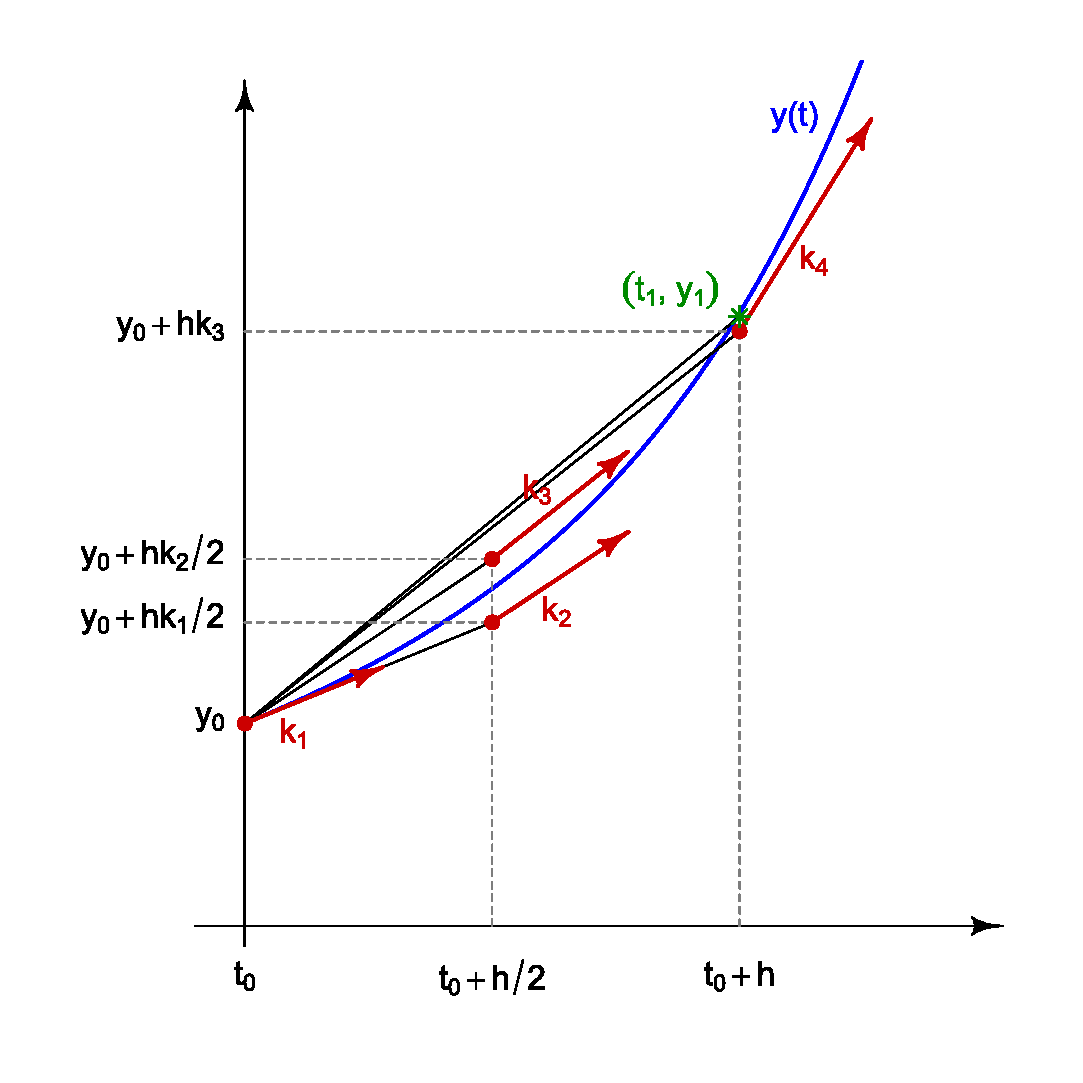
\includegraphics[width=0.45\linewidth]{slike/Runge_Kutta_slopes.eps}
			\caption{}
			\label{fig:RK4}
		
		\caption{Vizuelizacija Runge-Kuta integracije \cite{rk4}}
	\end{figure}
	
	
	
	
	
	
	\clearpage
	
	% Rekao bih da ponasanje u otvorenoj sprezi nije neophodno, u pitanju je klatno
	%\subsection{Ponašanje sistema u otvorenoj sprezi}
	
	
	
	%\clearpage 
	\subsection{Linearizacija sistema}
	\label{sec:linearizacija}
	
	Nelinearni model (\ref{eq:nonModel}) se može linearizovati razvijanjem u Tejlorov red u okoline tačke $(\vect{\bar{x}}, \bar{u})$:
	\begin{equation}
		\mathbf{f}(\mathbf{x}, u) \approx \mathbf{f}(\mathbf{\bar{x}}, \bar{u}) + \nabla_{\vect{x}} \mathbf{f}|_{(\vect{\bar{x}},\bar{u})} (\mathbf{x} - \mathbf{\bar{x}}) + \frac{\partial \mathbf{f}}{\partial u}|_{(\mathbf{\bar{x}},\bar{u})} (u - \bar{u}). \label{eq:linearization}
	\end{equation}
	
	Neka su $\vect{A} = \nabla_{\mathbf{x}} \mathbf{f}|_{(\bar{\mathbf{x}},\bar{u})}$, $B = \frac{\partial \mathbf{f}}{\partial u}|_{(\bar{\mathbf{x}},\bar{u})}$, $\Delta \mathbf{x} = \mathbf{x} - \bar{\mathbf{x}}$, i $\Delta u = u - \bar{u}$.
	Prethodna jednačina se može napisati kao:
	\begin{equation}
		\dot{\mathbf{x}} \approx \vect{A}\Delta \mathbf{x} + B\Delta u + \vect{f}(\bar{\mathbf{x}}, \bar{u}). \label{eq:linearized_system}
	\end{equation}
	
	Linearizacija se obavlja za različite $\bar{\mathbf{x}}$ čime se dolazi do porodice linearnih modela. Linearni model u okolini tačke  $\vect{f}(\vect{\bar{x}} = \vect{0}, u = 0) = \vect{0}$, može se napisati kao:
	\begin{align}
		\begin{split}
			\vect{\dot{x}}(t) &= A\vect{x}(t) + Bu(t) \\
			y(t) &= C\vect{x}(t) + Du(t)
		\end{split},
		\label{eg:lin_mod}
	\end{align}
	
	
	gde  $\vect{x}$, $u$, i $y$ označavaju odstupanje od ravnotežnog stanja. 
	\[
	\mathbf{A} =
	\begin{bmatrix}
		0 & 1.0000 & 0 & 0 & 0 \\
		0 & -0.0174 & 20.7861 & -0.0023 & 57.5344 \\
		0 & 0 & 0 & 1.0000 & 0 \\
		0 & -0.0174 & 63.8319 & -0.0071 & 57.4388 \\
		0 & -232.0252 & 0 & 0 & -755.4250
	\end{bmatrix}
	\]
	
	\[
	\mathbf{B} =
	\begin{bmatrix}
		0 \\
		0 \\
		0 \\
		0 \\
		333.3367
	\end{bmatrix}
	\]
	
	\[
	\mathbf{C} =
	\begin{bmatrix}
		1 & 0 & 0 & 0 & 0 \\
		0 & 0 & 1 & 0 & 0
	\end{bmatrix}
	\]
	
	\[
	\mathbf{D} =
	\begin{bmatrix}
		0 \\
		0
	\end{bmatrix}.
	\] \\[16pt]
	
	
	\subsubsection{Kontrolabilnost} \label{sec:kontrolabilnost}
	
	Kontinualni linearni sistem se smatra potpuno kontrolabilnim ako i samo ako iz početnog stanja, uz odgovarajući ulaz $u(t)$ sa $0 < t \leq t_f$ i konačnim horizontom $t_f$, može da se postigne
	proizvoljno stanje $\vect{x}(t_f) = \vect{x_f}$. \\
	
	Linearni sistem je potpuno kontrolabilan ako matrica kontrolabilnosti
	\begin{align}
		\vect{C}[\vect{A}, \vect{B}] = \begin{bmatrix}
			\vect{B} & \vect{A}\vect{B} & \vect{A}^2\vect{B} & \cdots & \vect{A}^{n-1}\vect{B}
		\end{bmatrix} 
	\end{align}
	
	ima pun rang $n$. \\
	
	\clearpage
	Kada se napon primeni na motor, stvara se struja i obrtni moment $\tau_1$ se stvara u centru rotacije horizontalne ruke. Na metalnom vratilu gde je klatno pričvršćeno, sila nastala od $\tau_1$ duž ruke $l_{e1}$ je horizontalna i pravolinijska u odnosu na oba $l_{e1}$ i $\tau_1$, u skladu sa opštom formulom:
	
	\begin{align}
		\vect{\tau} = \vect{r} \times \vect{F}. \quad 
	\end{align}
	
	Obrtni moment u centru mase klatna takođe je dat ovom formulom, iz kojeg se može izraziti amplituda $\tau_2$ kao funkcija ugla $\beta$:
	
	\begin{align}
		\tau_2 = l_{cm2} F \cos \beta, \quad
	\end{align}
	
	
	gde je $l_{cm2}$ rastojanje između metalnog vratila i centra mase klatna. Iz gornjih jednačina jasno je da je ulaz, napon primenjen na motor, direktna akcija na sve stanja sistema - struju motora, položaj i brzinu horizontalne ruke, kao i položaj i brzinu klatna. Postoji izuzetak za $\cos \beta = 0$, tj. kada je klatno horizontalno. U ovom slučaju, položaj i vektorske sile su paralelni, te stoga nije moguće primeniti obrtni moment. Stoga, varijable klatna nisu kontrolabilne u ovom trenutku. \\[16pt]
	
	
	\subsubsection{Opservabilnost}
	
	Kontinualni sistem se smatra potpuno opservabilnim ako je poznavanje $\vect{y}(t)$ za $0 \leq t \leq t_1$, sa $t_1$ konačnim, dovoljno za određivanje početnog stanja $\vect{x(0)}$. \\
	
	Linearni sistem je opservabilan ako matrica
	
	\begin{align}
		\vect{O}(\vect{A}, \vect{C}) = \begin{bmatrix}
			\vect{C} \\
			\vect{C}\vect{A} \\
			\vect{C}\vect{A}^2 \\
			\vdots \\
			\vect{C}\vect{A}^{n-1}
		\end{bmatrix} \quad
	\end{align}
	ima pun rang $n$. \\[16pt]
	
	\subsubsection{Stabilnost}
	
	
	
	Tačka \(\vect{\bar{x}}\) dinamičkog sistema se klasifikuje kao Ljapunov stabilna ako važi:
	\begin{align}
		\forall \epsilon > 0, \exists \delta > 0 : ||\vect{x(0)} - \vect{\bar{x}}|| < \delta \land t > 0 \Rightarrow ||\vect{x}(t) - \vect{\bar{x}}|| < \epsilon, \quad 
	\end{align}
	i asimptotski stabilna ako dodatno važi:
	
	\begin{align}
		\exists \epsilon > 0 : ||\vect{x(0)} - \vect{\bar{x}}|| < \epsilon \Rightarrow \lim_{t \to \infty} \vect{x}(t) = \vect{\bar{x}}. \quad
	\end{align}
	
	Asimptotska stabilnost nelinearnog sistema može se proceniti linearnizovanim sistemima dobijenim kod svake fiksne tačke pomoću Ljapunovljeve indirektne metode. Moguće je zaključiti da, za linearnizovani sistem (\ref{eg:lin_mod}):
	\begin{enumerate}
		\item ako sve sopstvene vrednosti matrice \(A\) imaju negativne realne delove, tada je fiksna tačka nelinearnog sistema stabilna;
		\item ako bar jedna sopstvena vrednost matrice \(A\) ima pozitivan realni deo, tada je fiksna tačka nelinearnog sistema nestabilna;
		\item ako nijedno od prethodno navedenog nije zadovoljeno, tj. ako bar jedna sopstvena vrednost leži iznad imaginarne ose, a nema sopstvene vrednosti sa pozitivnim realnim delom, onda se ne može izvesti zaključak.
	\end{enumerate} 
	
	
	
	\begin{table}[H]
		\centering
		\caption{Sopstvene vrednosti linearizovanih modela, asimptotska stabilnost redukovanog sistema ($X_2, \cdots, X_5$), kontrolabilnost i observabilnost za 5 tačaka, gde su sve promenljive stanja postavljene na nulu, osim $X_3$.}
		\label{table:eigenvalues}
		\begin{tabular}{c c c c c c c}
			\hline
			$X_3$ & Sopstvene vrednosti & Stabilan & Kontrolabilan & Observabilan \\
			\hline
			0 & $-737.2$, $-19.4$, $+7.0$, $-5.8$, $0$ & Ne & Da & Da \\
			$\pi/4$ & $-743.2$, $-11.8$, $-5.3$, $+5.0$, $0$ & -- & Da & Da \\
			$\pi/2$ & $-746.2$, $-9.1$, $-0.0$, $0$, $0$ & -- & Ne & Da \\
			$3\pi/4$ & $-743.2$, $-12.4$, $+0.1 + 5.0i$, $+0.1 - 5.0i$, $0$ & -- & Da & Da \\
			$\pi$ & $-737.2$, $-17.0$, $-0.5 + 6.8i$, $-0.5 - 6.8i$, $0$ & Da & Da & Da \\
			\hline
		\end{tabular}
		\label{tab:5_tacaka}
	\end{table}
	
	U tabeli \ref{tab:5_tacaka} je prikazana analiza za 5 različitih tačaka, čime se pokazuje da je $x_3 = 0$ (kada se sistem se nalazi u gornjem položaju) nestabilno stanje, ali ispunjava uslove kontrolabilnosti i opservabilnosti. 
	\\[16pt]
	
	\subsection{Poremećaji u sistemu}
	
	 U radu \cite{inicijalna} autor razmatra samo jedan izvor poreme\'caja i to step promenu stanja $\beta$. Razlog se ne navodi, ali je jasno da od 5 stanja datog sistema na stabilnost najve\'ci uticaj ima stanje $\beta$. U sekciji (\textbf{\ref{sec:kontrolabilnost}}) se razmatra uticaj stanja $\beta$ na kontrolabilnost sa stanovni"stva fizike. \\
	 
	 Pored analiziranog izvora poreme\'caja ima smisla razmotriti step promenu stanja $\alpha$ kao i impulsnu promenu stanja $i$. Razlog za razmatranje impulsnog poreme\'caja u slu"caju struje $i$ je taj "sto su vremenske konstante elektri"cnih sistema za red veli"cine manje od vremenskih konstanti mehani"ckih sistema. Odnosno na step promenu struje jako brzo odreaguju kontroleri projektovani za stabilizaciju napona, pa to eksterno deluje kao impulsni poreme\'caj u struji. \\
	 
	 Tokom simuliranja projektovanih kontrolera razmatraju se step promena stanja $\beta$ inteziteta +10$^o$ i -10$^o$. \\[16pt]
	 

	\subsection{Upravljački signali i ograni"cenja signala}
	
	Upravlja"cki signal za razmatrani sistem je napon $u$ motora koji je zadu"zen za rotaciju horizontalne sekcije klatna. Autor u radu \cite{inicijalna} navodi slede\'ca ograni"cenja:
	
	\begin{itemize}
		\item Napon motora $u \in [-6, 6] ~\text{V}$, me\dj utim svi grafici autora prikazuju opseg $u \in [-5, 5] ~\text{V}$. U radu se usvaja vrednost sa grafika autora.
		\item Vertikalni ugao  $\beta \in [-12, 12] ~\text{°}$
		\item Horizontalni ugao  $\alpha \in [-180, 180] ~\text{°}$
	\end{itemize}
	
	\clearpage
	
	
	\section{Projektovanje sistema upravljanja}
	
	Projektovanje sistema upravljanja se sastoji iz dva dela: generisanje željene trajektorije i projektovanje kontrolera koji treba da isprati željenu trajektoriju i održava sistem u gornjem položaju. \\
	
	Često je korisno dizajnirati trajektorije van mreže, tj. definisati putanju u prostoru stanja koju sistem treba da izvede unapred. U takvoj situaciji nismo ograničeni vremenom ili računski potrebnom snagom da se izvrše proračuni tokom samog procesa, što je posebno korisno kod složenih sistema sa brzom dinamikom. Putanje se dizajniraju koristeći model sistema, analizirajući njegov odgovor na dostupne ulaze. Ova strategija se široko koristi u robotici, gde postoji potreba za planiranjem kretanja mobilnih robota u ograničenim prostorima \cite{inicijalna}. \\
	
	Jedan od pristupa za generisanje trajektorije je optimalno upravljanje,  koje se bavi problemom određivanja ulaza dinamičkog sistema koji opitmizuje (maksimizuje ili minimizuje) odredjenu funkciju troška koja govori o performansama sistema. Sa odgovrajućom funkcijom troška mogu se odrediti putanja i zakon upravljanja koji zadovoljava zahteve projektovanja. Takodje, većina nelinearnih problema se može rešiti oslanjanjem na numeričke metode. U radu se \cite{inicijalna} kao alternativa optimizacionim metodama predla"zu ad hoc strategije gde se implicitno formira upravljanje na bazi upravljanja veli"cina kao "sto je energija sistema. \\
	
	Nakon što se izgeneriše trajektorija, potrebno je isprojektovati kontroler koji će pratiti zadatu putanju. U radu \cite{inicijalna} se predla"zu dve metode za stabilizaciju klatna. Prvi pristup podrazumeva projektovanje globalnog LQR kontrolera na osnovu linearizovanog modela u ravnote"znom stanju. Mana ovog pristupa je to "sto se karakteristike sistema zna"cajno menjaju u zavisnosti od polo"zaja klatna, pa bi ovakav kontroler morao da ima lo"se performanse zbog ve\'ce potrebe za robusno"s\'cu. Drugi pristup podrazumeva projektovanje niza lokalnih LQR kontrolera za odre\dj ene sekcije du"z trajektorije. Prednost ovog pristupa je to "sto se mogu posti\'ci bolje performanse usled ve\'ce robustnosti sistema du"z trajektorije.  \\[16pt]
	

	\subsection{Generisanje trajektorije}\label{sec:gen_traj}
	
	Ovo poglavlje istražuje kako pronaći optimalan ulaz za dinamički sistem, omogućavajući mu da sledi željenu putanju u prostoru stanja. Ova putanja treba da bude u skladu sa zadanim ograničenjima i optimizuje zadatu veličinu. Iako se različite strategije mogu koristiti za projektovanje putanja, fokus je stavljen na optimalno upravljanje. Ova tehnika pruža jasan okvir za pronalaženje rešenja za probleme podložne ograničenjima i ciljevima optimizacije. Pored optimalnog generisanja trajektorije, implementirane su i ad hoc metode za uspravljanje klatna kao alternativno i jednostavno rešenje. 
	
	\subsubsection{Ad hoc strategije}
	\label{sec:andhoc}
	
	Jedna od najčešće korišćenih metoda za podizanje FP je kontrola energije. U ovom slučaju se energija sistema kontroliše umesto direktnog kontrolisanja pozicije i brzina klatna \cite{inicijalna}.
	U \cite{energy_c} predložen je zakon upravljanja za uspravljanje klatna zasnovanoj na kontroli energije (eng \textit{Energy control}): \\
	
	\begin{equation}
		u = \operatorname{sat}\left[k_v (E - E_0)\right] \operatorname{sign}( \dot{\beta} \cos \beta), 
		\label{eq:en_control}
	\end{equation} \\
	
	
	gde su $\textit{E}$ trenutna energija sistema, 
	$\textit{E}_0$ je željena energija sistema, $\textit{k}_v$ je pojačanje kontrolera, a $\beta$ je ugao penduluma. Prvi pojam definiše amplitudu ulaza. Može se posmatrati kao proporcionalni kontroler, gde je promenljiva razlika u energiji između trenutnog stanja i energije ciljnog stanja, koja je konvencionalno postavljena na nulu. Amplituda je ograničena zbog fizičkih ograničenja aktuatora. Drugi pojam definiše znak upravljačkog ulaza i obezbeđuje da je efekat ulaza dodavanje energije sistemu. Član $\cos \beta$ procenjuje da li je trenutni položaj penduluma iznad ili ispod horizontalnog položaja. Za $\cos \beta = 0$, pendulum je horizontalan, stoga sistem nije kontrolabilan - nema prenosa energije na pendulum. Sa dodatnim članom $\dot{\beta}$, sila se primenjuje protiv smera kretanja penduluma kada je ispod horizontalnog položaja i u istom smeru kada je iznad.\\
	
	Važno je napomenuti da je ovaj zakon upravljanja projektovan specifično za sistem FP, stoga nije vrlo opšte primenljiv. Takođe, ograničen je na situacije gde nivo energije ciljnog stanja nije degenerisan. Iako će kontroler dovesti sistem do stanja sa određenom energijom, ako postoji više konfiguracija sa istom energijom, nije moguće izabrati između njih. Ovo je slučaj kod FP, gde energija sistema ne zavisi od ugla horizontalne ruke $\alpha$. Dakle, ovom tehnikom nema kontrole nad ovom varijablom tokom uspravljanja. \\
	
	Zakon upravljanja definisan u jednačini (\ref{eq:en_control}) zahteva izračunavanje energije sistema. Modifikovana verzija kontrolera predložena je u \cite{energy_c} koja uzima u obzir samo varijable prostora stanja. Ovaj zakon upravljanja poznate je kao 
	\textit{exponentiation of the pendulum position} i glasi:\\
	
	\begin{equation}
		u = \operatorname{sat}(k_v |\beta^n|) \operatorname{sign}( \dot{\beta} \cos \beta).
	\end{equation} \\
	
	U ovom slučaju, prvi član je modifikovan, sada uzimajući ugao između trenutnog položaja i vertikale.
	Dodaje se eksponent \textit{n} izražen u izrazu, što povećava amplitudu ulaza kada je pendulum daleko od uspravnog položaja, ali je manja kada je bliže. U \cite{inicijalna} navode da ovaj zakon omogućava glađi prelaz između nelinearnog upravljanja i upravljanja koji balansira klatno u gornjem položaju. Drugi član ostaje nepromenjen. \\
	
	U \cite{ener_shaping} je izveden i testiran zakon upravljanja poznat kao \textit{energy shaping}. Pomenuti zakon upravljanja je izveden na osnovu inverznog klatna koji rotira samo oko vertikalne ose i glasi: \\
	
	\begin{equation}
		u = \operatorname{sat}(k_1 (\dot\alpha + k_2 \cos(\beta) \dot\beta)).
	\end{equation}
	
	\subsubsection{Optimalno upravljanje}
	Optimalna kontrola se bavi problemom određivanja ulaza dinamičkog sistema koji optimizuju, tj. minimiziraju ili maksimiziraju, određeni indeks performansi. Sa odgovarajućim izborom funkcije troška, mogu se odrediti trajektorije i zakoni upravljanja tako da zadovolje zahteve dizajna.\\
	
	U ovom radu, koristili smo model prediktivnog upravljanja (engl. \emph{Model Predictive Control}, MPC) kao pristup za optimalnu kontrolu. \\
	
	MPC koristi matematički model sistema kako bi predvidio buduće ponašanje sistema na osnovu trenutnog stanja i unapred zadatih referenci. Model može biti linearni ili nelinearni, ali je ključno da bude dovoljno tačan za predviđanje sistema u predvidjenom vremenskom horizontu. MPC optimizuje kontrolne akcije za određeni horizont vremena unapred. MPC ne razmatra samo trenutno stanje sistema, već razmatra niz budućih koraka, obično u diskretnim vremenskim koracima. Ovaj horizont može biti kratkoročan ili dugoročan, u zavisnosti od zahteva sistema i dinamike procesa. MPC minimizira ili maksimizira funkciju cilja koja predstavlja kriterijum performansi sistema. To može uključivati minimizaciju greške u praćenju referenci, minimizaciju potrošnje energije ili slične ciljeve. MPC primjenjuje samo prvu kontrolnu akciju iz optimizacionog problema, nakon čega se proces ponavlja u svakom diskretnom vremenskom koraku. Ovaj pristup omogućava MPC-u da reaguje na promene u stanju sistema i spreči akumulaciju grešaka. Njegova sposobnost da predviđa buduće stanje sistema i optimizuje kontrolne akcije čini ga moćnim alatom za upravljanje sistemima sa kompleksnom dinamikom i nelinearnostima \cite{mpc}.\\
	
	
	\begin{figure}[!htb]
		\centering
		\begin{subfigure}{0.5\linewidth}
			\centering
			\includegraphics[width=\linewidth]{slike/mpc_sc.png}
			\caption{}
			\label{fig:mpc_sc}
		\end{subfigure}
		\hfill
		\begin{subfigure}{0.48\linewidth}
			\centering
			\includegraphics[width=\linewidth]{slike/mpc.png}
			\caption{}
			\label{fig:mpc_f}
		\end{subfigure}
		\caption{(a) Šema MPC-a, (b) ilustracija rada MPC-a \cite{mpc} }
	\end{figure}
	
	
	U radu \cite{inicijalna} autor razmatra primenu optimizacionih metoda nad pojednostavljnim sistemom $\ddot{\alpha}(t) = \omega_0^2 \operatorname{sin}\alpha(t) + u(t)$. Vr"si se direktna optimizacija Hamiltonijana oblika $H(u) = \vect{\lambda}^T(t)\vect{f}(\mathbf{x}(t), u(t)) + \mathcal{L}(\mathbf{x}(t), u(t))~\operatorname{d}t$, gde je $\mathcal{L}(\mathbf{x}(t), u(t))$ lagran"zijan sistema. Lagran"zijan sistema tipi"cno reprezentuje energiju sistema i ima slede\'ci oblik: $\mathcal{L}(\mathbf{x}(t), u(t)) = \frac{1}{q}||\mathbf{x}(t)||_{\mathbf{Q}}^q + \frac{1}{p}||u(t)||_{W}^p$. Prilikom analize ovog sistema autor ne specificira $\mathbf{Q}$, ali se navodi primena $q=2$ norme nad stanjima i primena $p=1$ i $p=2$ norme nad upravljanjem. Primena $p=1$ norme rezultuje upravljanjem koje je "cesto u zasi\'cenju i naglo menja polaritet dok $p = 2$ norma favorizuje glatko upravljanje. \\
	
	U op"stem slu"caju odre\dj ivanje optimalnog upravljanja za nelinearni sistem $\dot{\vect{x}}(t) = \vect{f}(\vect{x}(t), \vect{u}(t))$ podrazumeva minimizaciju funkcije tro"ska $J(\mathbf{u}(t)) = \Psi(\mathbf{x}(t)) + \int_{t_0}^{T}\mathcal{L}(\vect{x}(t), \vect{u}(t))~\operatorname{d}t$, pod ograni"cenjem da je zadovoljena dinamika sistema $\dot{\vect{x}}(t) = \vect{f}(\vect{x}(t), \vect{u}(t))$, upravljanje je u dozvoljenim granicama $\mathbf{u}(t)\in \mathbf{\mathcal{U}}$, kao i stanja $\mathbf{x}(t)\in \mathbf{\mathcal{X}}$.  Ovaj optimizacioni problem se re"sava primenom Pontrjaginovog principa maksimuma, odnosno optimalno opravljanje $\vect{u}^*(t)$ je mogu\'ce odrediti minimizacijom Hamiltonijana $H(\vect{u}(t)) = \vect{\lambda}^T(t)\vect{f}(\mathbf{x}(t), \vect{u}(t)) + \mathcal{L}(\mathbf{x}(t), \vect{u}(t))$. Sprovo\dj enje ovog postupka minimizacije podrazumeva re"savanje sistema nelinearnih diferencijalnih jedna"cina: 
	\begin{align}\label{eq:Hamilton}
		\dot{\vect{\lambda}}(t) &= -\nabla_{\vect{x}}H\\
		\dot{\vect{x}}(t) &= \nabla_{\vect{\lambda}}H~~.
	\end{align}
	Sistem jedna"cina (\ref{eq:Hamilton}) je poznat kao i Hamiltonov sistem jedna"cina. Druga jedna"cina je ispunjena zbog dinamike sistema, pa se problem svodi na re"savanje:
	\begin{equation}		\dot{\vect{\lambda}}(t) = -{\vect{\lambda}}^T(t)\vect{f}_{\mathbf{x}}(\mathbf{x}(t), u(t)) - \mathcal{L}_{\mathbf{x}}(\mathbf{x}(t)),
	\end{equation} 
	uz po"cetni uslov $\vect{\lambda}^T(t) = \Psi_{\mathbf{x}}(\mathbf{x}(T))$.\\
	
	U ovom radu za potrebe pronala"zenje optimalne trajektorije primenjujemo MPC implementiran pomo\'cu biblioteke za optimalno upravljanje \cite{CASADI}. Ovaj softverski paket omogu\'cuje korisniku da formuli"se optimizacione probleme, dok se re"savanje prosle\dj uje namenskim bibliotekama za re"savanje optimizacionih problema napisanih u C programskom jeziku. \\
	
	 Formulacija MPC za potrebe nala"zenja optimalne trajektorije, odnosno optimalnog upravljanja, se razlikuje u zavisnosti od metode koja se koristi za re"savanje optimizacionog problema. U ovom radu se primenjuje \emph{multiple shooting} metoda. Ova metoda pripada familiji direktnih za re"savanje problema optimalnog upravljanja. \emph{Multiple shooting} podrazumeva diskretizaciju stanja sistema kao i upravljanja, a zatim re"savanje optimizacionog minimizacijom cene $J(\mathbf{u}(t))$ pod uslovom da su parcijalne trajektorije na granicama kontinualne. Odnosno na intervalu $t\in[t_i, t_{i+1}]$ se re"sava diferencijalna jedna"cina:
	\begin{align}\label{eq:mutiple_shooting}
		\dot{x}_i(t; s_i; u_i) &= f(x_i(t; s_i; u_i)) \\
		x_i(t; s_i; u_i) &= s_i,
	\end{align}
	pri "cemu je $s_i$ ve"sta"cka promenljiva koja se uklju"cuje u proces optimizacije. Re"savanjem diferencijalnih jedna"cina (\ref{eq:mutiple_shooting}) se izdvaja deo trajektorije $x_i(t; s_i; u_i)$ na intervalu $t\in[t_i, t_{i+1}]$. Na osnovu dobijene trajektorije se mo"ze izra"cunati parcijalna cena $j_i(x_i(t; s_i; u_i), u_i) = \int_{t_i}^{t_{i+1}}\mathcal{L}(x_i(t; s_i; u_i), u_i)~\operatorname{d}t$. Kona"cno mo"ze se formirati optimizacioni problem kao:
	\begin{equation}\label{eq:multiple_minimize}
		\min_{\mathbf{s}, \mathbf{u}} \sum_{i=0}^{N-1} j_i(x_i(t; s_i; u_i), u_i) + E(s_N), \\
	\end{equation}pod uslovom:
	\begin{align}
		s_0 - x_0 &= 0\\
		s_{i+1} - x_i(t_{i+1}; s_i; u_i) &= 0\\
		h(s_i, u_i) &\geq 0\\
		r(s_N) &\geq 0 ~~,
	\end{align} gde $h(s_i, u_i)$ i $r(s_N)$ predstavljaju ograni"cenja nad trajektorijom i krajem trajektorije. \cite{multiple_shooting}\\
	
	Prilikom implementacije MPC primenom \cite{CASADI} paketa definisani su slede\'ci parameti:
	\begin{itemize}
		\item Funkcija cene: $J = \gamma_1||\mathbf{x}(T)||^2_{\mathbf{Q}_T} + \sum_{i = 0}^{N-1}\gamma_2||\mathbf{x}(t_i)||^2_{\mathbf{Q}} + \gamma_3||u(t_i)||^2_{R}$.
		\item Horizont predikcije $N = 1500$.
		\item Matrice $\mathbf{Q}_T$, $\mathbf{Q}$ i skalar $R$ su izabrani tako da normalizuju stanja, odnosno upravljanje. 
		\item Koficijenti skaliranja: $\gamma_1 = 0.1N$, $\gamma_2=0$, $\gamma_3=1$. 
		
	\end{itemize}, 
	 Prilikom primene \emph{multiple shooting} metode neophodno je izra"cunavanje $x(t_{i+1}; s_i; u_i)$ na osnovu po"cetne ta"cke trajektorije $s_i$, za te potrebe se primenjuje RK4 numeri"cka integracija sa korakom 1ms. \\
	
	Zbog problema sa konvergencijom u ovom radu su uvedene tri modifikacije:
	\begin{itemize}
		\item Ispituje je se samo $p=2$ norma.
		\item Matrica $\mathbf{Q}_T$ je svuda nula osim za stanja $\alpha$ i $\beta$.
		\item U funkciji cene se ne koristi "clan $\gamma_2||\mathbf{x}(t_i)||^2_{\mathbf{Q}}$, pokazalo se da lo"se uti"ce na konvergenciju. Razlog za to mo"ze biti to "sto u odre\dj enim delovima trajektorije treba da pove\'camo amplitudu svih stanja kako bi uspe"sno uspravili klatno.
	\end{itemize}
	
	
	
	
	
	
	
	
	
	
	
	 
	
	
	\newpage
	\subsection{Projektovanje kontrolera}\label{sec:LQR}
	
	Nakon generisanja referentnih trajektorije potrebno je projektovati kontroler čiji je zadatak da u što većoj meri isprati željenu trajektoriju i kontroler koji će održavati sistem u željenom, gornjem položaja. \\
	
	Linearni kontroleri su validni samo u onom regionu gde je izvršena linearizacija sistema, a kako je zadatak upravlanje nelineranim sistemom potrebno je napraviti ansambl kontrolera. \\
	
	U radu \cite{inicijalna} su se bavili projektovanjem LQG kontrolera. Kalman filter je optimalan za procenu stanja u linearnim sistemima, ali kada se primeni na nelinearne sisteme, može doći do netačnih procena stanja zbog odstupanja između stvarne nelinearnosti sistema i linearnog modela koji se koristi u Kalman filtru. Iz ovog razloga, u ovom radu smo se zadržali na korišćenju LQR kontrolera. \\
	
	LQR (Linear Quadratic Regulator) je metoda optimalne kontrole koja se koristi za pronalaženje kontrolnih ulaza koji minimizuju određenu kvadratnu funkciju troška. LQR nudi nekoliko prednosti, uključujući jednostavnu implementaciju i robustnost, dok osigurava stabilnost sistema pod određenim uslovima. LQR kontroler ima nekoliko poželjnih svojstava, na primer, održava red sistema, ima faznu marginu od najmanje 60 stepeni i beskonačnu marginu pojačanja.\\
	
	Da bi se primenio LQR na sistem, dve osobine koje mora da zadovolji sistem je da bude kontrolabilan i opservabilan u okolini tačke gde je izvršena linearizacija sistema. Na osnovu analize prikazane u tabeli \ref{tab:5_tacaka} zaključuje se da jedino u slučaju kada je klatno u horizontalnom položaju ($\beta$ = $\pi /2$) nije moguće primeniti LQR kontroler.\\
	
	
	Cilj algoritma LQR je pronaći vektor pojačanja $\vect{K}$ za zakon povratne sprege u prostoru stanja
	\begin{equation}
		\vect{u} = -\vect{K}\vect{x}, 
	\end{equation}
	
	koji se primenjuje na kontinualni linearni sistem, definisan u (\ref{sec:linearizacija}), \\
	
	\begin{equation}
		\begin{cases}
			\dot{\vect{x}}(t) = \vect{A}\vect{x}(t) + \vect{B}\vect{u}(t) \\
			\vect{y}(t) = \vect{C}\vect{x}(t) + \vect{D}\vect{u}(t)
		\end{cases}, 
	\end{equation}\\
	
	a minimizuje funkciju troška\\
	
	\begin{equation}
		\vect{J} = \int_{0}^{\infty}  \vect{x}^T \vect{Q}_r \vect{x}  + \vect{u}^T \vect{R}_r \vect{u} \operatorname{d}t~~.
	\end{equation} \\
	
	Matrice $\vect{Q}_r$ i $\vect{R}_r$ određuju relativni značaj koji se pridaje regulaciji stanja i trošku ulaza, i treba ih odabrati uzimajući u obzir ciljeve dizajna sistema. Matrica $\vect{P}$ se dobija rešavanjem Rikatijeve jednačine: \\
	\begin{equation}
		\vect{A}^T \vect{P} + \vect{P} \vect{A} - \vect{P} \vect{B} \vect{R}^{-1} \vect{B}^T \vect{P} + \vect{Q}_r = \vect{0}, 
	\end{equation} \\
	
	nakon čega se računa pojačanje $K$ kao:
	\begin{equation}
		\vect{K} = \vect{R}_r^{-1}\vect{B}\vect{P}.
	\end{equation}
	
	\begin{figure}[!h]
		\centering
		\includegraphics[width=0.6\linewidth]{slike/lqr.jpg}
		\caption{Blok dijagram feedback kontrolera \cite{inicijalna}}
		\label{fig:lqr}
	\end{figure}
	
	
	
	Prelazak između kontrolera vrši se u dva različita režima rada: \\
	
	1. Kontrola za podizanje sistema primenjuje se direktno na uređaj. Samo linearni kontroler oko krajnje tačke je aktivan (globalni LQR kontroler). Tranzicija između režima uspravljanja sistema i režima ravnoteže oko uspravnog poožaja se dešava kada se ugao penduluma dovoljno približi nultom položaju ($\beta$ < 18$^\circ$). Ovaj pristup se koristi kada nema referentne putanje, i podizanje sistema se izvodi u zatvorenoj petlji, na primer sa Ad hoc strategijama opisanim u \ref{sec:andhoc}. \\
	
	2. Referentna kontrola se primenjuje na uređaj, koji zauzvrat ima zatvoreni skup linearnih kontrolera koji stabilizuju razliku između izvedene putanje i referentne putanje. Ovo se naziva Gain Scheduling controller.\\
	
	Gain Scheduling kontroler implementiran u upravljanju FP bira jedan od šest kontrolera koji se koristi u skladu sa trenutnim uglom $\beta$. Važno je napomenuti da su oni raspoređeni simetrično: prvi član Tejlorovog reda je identičan za $\beta = \pm \theta$, pa je i inkrementalni model isti. 
	Na slici (Sl. \ref{fig:ganSc}) su prikazani regioni rada \emph{gain scheduling} kontrolera, u funkciji ugla $\beta$ ($x_3$). Tačke označavaju mesta gde je izvedena Jakovijeva linearizacija, a $C_1$ do $C_6$ označavaju kontrolere koji rade u tom konkretnom regionu. Na primer $C_1$ radi za $\beta \in [-18^\circ, 18^\circ]$, i odgovoran je za održavanje klatna u uravnoteženom položaju na gore.
	
	\begin{figure}[!h]
		\centering
		\includegraphics[width=0.5\linewidth]{slike/gainSc.jpg}
		\caption{Gain Scheduling kontroler \cite{inicijalna}}
		\label{fig:ganSc}
	\end{figure}
	
	Svaki LQR kontroler, koji je dizajniran nezavisno, koriguje vrednost ulazne promenljive kako bi aproksimirao ponašanje stvarnog sistema prema onom predviđenom u referentnoj putanji.\\
	
	\subsubsection{\emph{Feedworward} LQR}
	LQR u bazi"cnoj formulaciji dovodi sistem u koordinatni po"cetak i nema mogu\'cnost pra\'cenja reference. Me\dj utim, u ovom radu je neophodno pratiti referencu. Ovaj problem se re"sava uvo\dj enjem modifikacije u algoritam koja efektivno predstavlja \emph{feedforward} dejstvo.\\
	
	Neka su $\vect{x}_r$ i $\vect{u}_r$ referetno stanje, odnosno referetno upravljanje. Referetno stanje i upravljanje prate dinamiku originalnog sistema odnosno va"zi:
	\begin{align}\label{eq:ss_feedforward}
		\vect{C}\vect{x}_r + \vect{D}\vect{u}_r &= \vect{r}\\
		\vect{A}\vect{x}_r + \vect{B}\vect{u}_r &= \dot{\vect{x}}_r~~.
	\end{align}
	Referenca je tipi"cno konstatna, pa se mo"ze usvojiti  $\dot{\vect{x}}_r = \vect{0}$. Jedna"cina (\ref{eq:ss_feedforward}) se mo"ze zapisati u matri"cnom obliku kao:

	
	
	\begin{equation}\label{eq:ss_ff_matrix}
		\begin{bmatrix} \vect{x}_r \\  \vect{u}_r \end{bmatrix} = 
		\begin{bmatrix} \vect{A} &  \vect{B} \\  \vect{C} &  \vect{D} \end{bmatrix}^{-1}
		\begin{bmatrix} \vect{0} \\  \vect{r} \end{bmatrix}~~.
	\end{equation} \vspace{1cm}
	
	Ako se na LQR dovede signal gre"ske u skladu sa slikom (Slika \ref{fig:archGain}) implicitno se vr"si transformacija koordinata $\hat{\vect{x}} = \vect{x} - \vect{x}_r, \hat{\vect{u}} = \vect{u} - \vect{u}_r$, gde su $\hat{\vect{x}}$ i $\hat{\vect{u}}$ stanje i upravljanje transformisanog sistema.
	
	\begin{figure}[!h]
		\centering
		\includegraphics[width=0.5\linewidth]{slike/applyLqr.jpg}
		\caption{Arhitektura Gain Scheduling kontrolera. Vektor $K_i$, $i \in \{1, \ldots, 6\}$ se bira u skladu sa trenutnim uglom klatna \cite{inicijalna}}
		\label{fig:archGain}
	\end{figure} 
	Primenom zakona upravljanja oblika $\hat{\vect{u}} = - \vect{K}\hat{\vect{x}}$ transformisani sistem dovodimo u koordinatni po"cetak, u tom slu"caju va"zi $\hat{\vect{x}} = \vect{0} \rightarrow \vect{x} = \vect{x}_r$. Zakon upravljanja iz transformisanog sistema mo"zemo zapisati kao $\vect{u} = -\vect{K}(\vect{x} - \vect{x}_r) + \vect{u}_r$. Ako primenimo izvedenu relaciju iz jedna"cine (\ref{eq:ss_ff_matrix}) mo"zemo zapisati:
	\begin{equation}
		\vect{u} = -\vect{K}\vect{x} + \begin{bmatrix} \vect{K} &  \vect{I} \end{bmatrix}
		\begin{bmatrix} \vect{A} &  \vect{B} \\  \vect{C} &  \vect{D} \end{bmatrix}^{-1}
		\begin{bmatrix} \vect{0} \\  \vect{I} \end{bmatrix} \vect{r}~~,
	\end{equation}
	odnosno:
	\begin{equation}\label{eq:ff_final}
		\vect{u} = -\vect{K}\vect{x} + \vect{F} \vect{r}~~.
	\end{equation}\\
	
	Zaklju"cak je da primenom zakona upravljanja u skladu sa slikom (Slika \ref{fig:archGain}) implicitno primenjujemo \emph{feedforward} dejstvo. Jo"s va"znije, u slu"caju da nam je na raspolaganju samo referenca $\mathbf{r}$ mogu\'ce je koristit LQR bez direktnog generisanja $\vect{x}_r$ i $\vect{u}_r$.
	
	
	
	

	
	
	
	
	
	
	
	\newpage
	
	
	\section{Komparativna analiza algoritama za uspravljanje klatna} \label{sec:comp}
	\subsection{Diskusija}
	
	U ovoj sekciji su predstavljeni rezultati simulacija pomo\'cu kojih su verifikovani isprojektovani algoritmi. Implementiran je globalni LQR kao i \emph{gain scheduling}. Primena razli"citih kontrolera za stabilizaciju nije rezultovala velikim razlikama u trajektorijama, zbog toga u sekciji (\ref{sec:grafici}) su prikazani samo grafici sa \emph{gain scheduling} kontrolerom za stabilizaciju. \\ 
	
	Sve trajektorije su generisane \emph{offline} primenom egzaktnog modela. Prilikom dovo\dj enja klatna u uspravan generisano upravljanje i trajektorija u prostoru stanja se koriste kao referenca. Robustnost na gre"ske u modeliranju je ispitana naknadnim uvo\dj enjem $5\sigma$ gre"saka u odnosu na vrednosti iz tabele \ref{tab:tab1}.\\
	
	Svi razmatrani algoritmi su uspe"sno doveli klatno u uspravan polo"zaj. U slu"caju primene globalnog LQR kontroler se uklju"cuje ako je ugao $|\beta| \leq 16^o$, dok je \emph{gain scheduling} uvek uklju"cen. Nakon "sto ugao $|\beta|$ dostigne granicu od $16^o$ referentna trajektorija se postavlja na nulu i stabilizacija klatna se u potpunosti prepu"sta kontroleru.\\
	
	Prilikom simulacije prisutan je merni "sum. Analiza uticaja mernog "suma je izostavljena zbog prirode LQR kontroler. U pitanju je kontroler sa "cistim proporcionalnim dejstvom i kao takav nema osobine potiskivanja "suma (za razliku od kontrolera sa integralnim dejstvom). Mogu\'ce je delimi"cno smanjiti osetljivost na "sum prilikom projektovanja uvo\dj enjem ve\'ce cene upravljanja.\\
	
	Kako bi uporedili algoritme za uspravljanje klatna uvedene su slede\'ce metrike:
	\begin{itemize}
		\item $t_{16^o}$ - trenutak kad ugao $|\beta|$ pre\dj e granicu od $16^o$.
		\item $t_s$ - vreme smirenja ugla $\beta$.
		\item $E_u$ - energija upravlja"ckog signala, koristi se L2 norma.
	\end{itemize}
	Rezultati simulacija su tabelarno prikazani u sekciji (\ref{sec:tab}).\\
	
	Radi testiranja rada kontrolera u prisustvu poreme\'caja simulirana je step promena ugla $\beta$ u iznosu $\pm10^o$. Poreme\'caj se uvodi tek nakon "sto klatno uspe"sno dostigne gornji polo"zaj. Zbog toga se u sekciji (\ref{sec:por}) prikazuje samo jedan grafik. Algoritam za uspravljanje nema uticaja na poreme\'caje nakon "sto se dosegne gornji polo"zaj, kao "sto ne postoji razlika me\dj u LQR i \emph{gain scheduling} kontrolerima u gornjem polo"zaju.\\
	
	Prilikom generisanja trajektorija kori"s\'cen je RK4 algoritam opisan u sekciji (\ref{sec:matlab_model}) bez dodatnog umanjenja koraka integracije. Me\dj utim, prilikom dinamike klatna korak integracije je smanjen 4 puta. Cilj ovog pove\'canja preciznosti je da se elimini"su gre"ske usled neadekvatnog koraka odabiranja. \\
	
	Analizom grafika iz sekcije (\ref{sec:grafici}) mogu se uo"citi slede\'ce sli"cnosti me\dj u generisanim upravljanjima:
	\begin{itemize}
		\item Upravljanje generisano primenom MPC kvalitativno ima oblik kao upravljanje generisano primenom \emph{energy shaping}
		\item Upravljanje generisano primenom \emph{energy control} kvalitativno ima oblik kao upravljanje generisano primenom \emph{exponentiation of the pendulum position}
	\end{itemize} 
	
	
	
	
	
	
	
	
	
	
	
	
	
	
	
	\clearpage
	\subsection{Rezultati simulacije} \label{sec:grafici}
	\begin{figure}[!h]
		\centering
		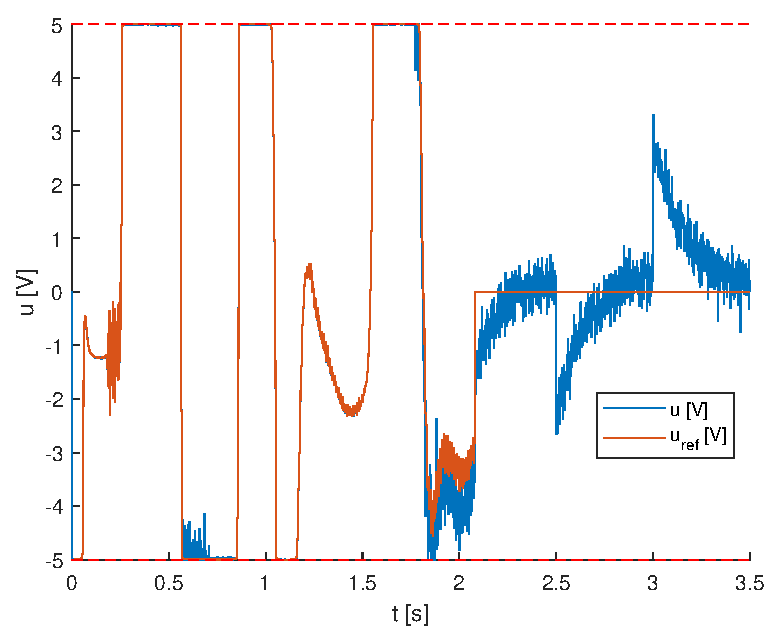
\includegraphics[width=0.6\linewidth]{slike/Control_MPC_trajectory_norm2.eps}
		\caption{Upravlja"cki signal generisan primenom MPC}
		\label{fig:cntrl_MPC}
	\end{figure}
	
	\begin{figure}[!h]
		\centering
		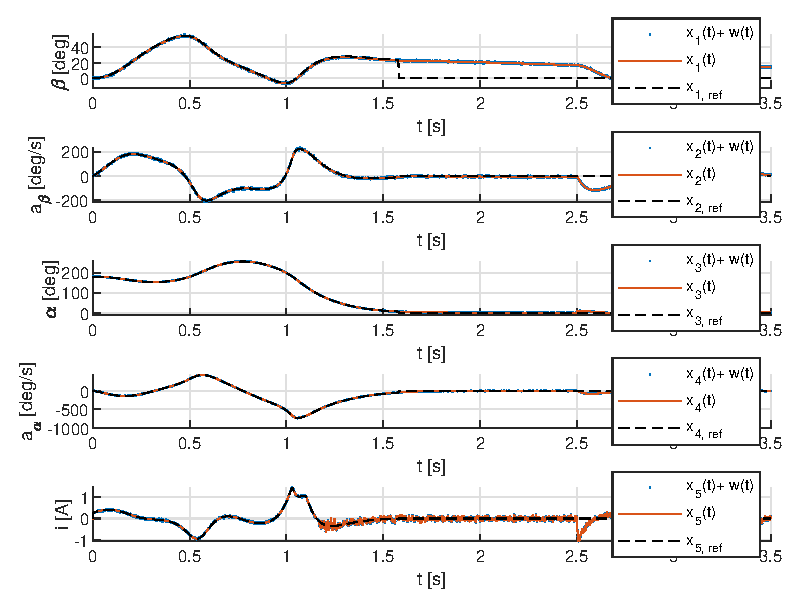
\includegraphics[width=.9\linewidth]{slike/States_MPC_trajectory_norm2.eps}
		\caption{Stanja sistema nakom primene upravljanja generisanog primenom MPC}
		\label{fig:traj_MPC}
	\end{figure}
	\clearpage
	
	\begin{figure}[!h]
		\centering
		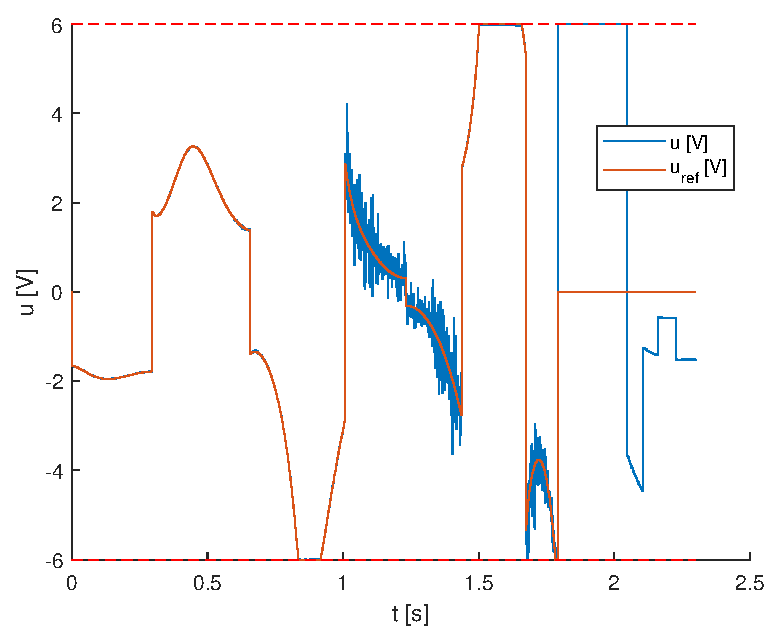
\includegraphics[width=0.6\linewidth]{slike/Control_EnergyControl_trajectory.eps}
		\caption{Upravlja"cki signal generisan primenom \emph{energy control}}
		\label{fig:cntrl_energycntrl}
	\end{figure}
	
	\begin{figure}[!h]
		\centering
		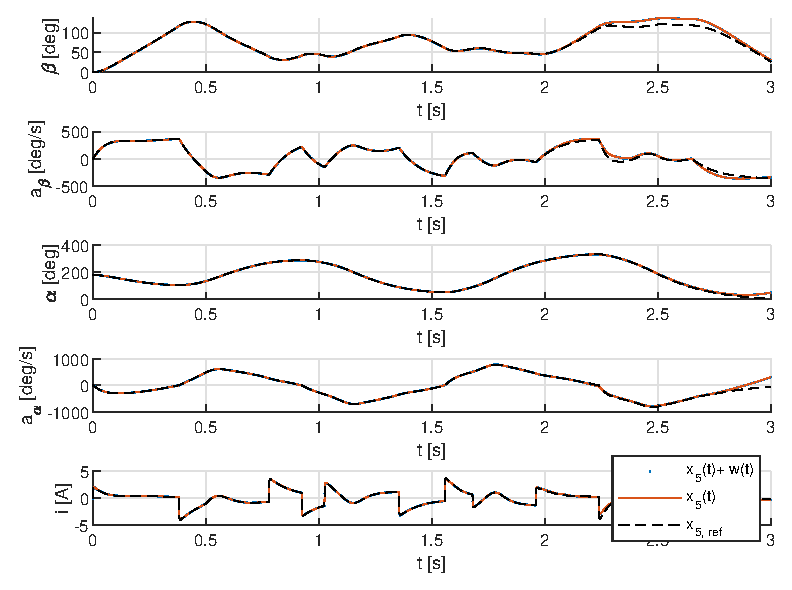
\includegraphics[width=.9\linewidth]{slike/States_EnergyControl_trajectory.eps}
		\caption{Stanja sistema nakom primene upravljanja generisanog primenom \emph{energy control}}
		\label{fig:traj_energycntrl}
	\end{figure}
	\clearpage
	
	\begin{figure}[!h]
		\centering
		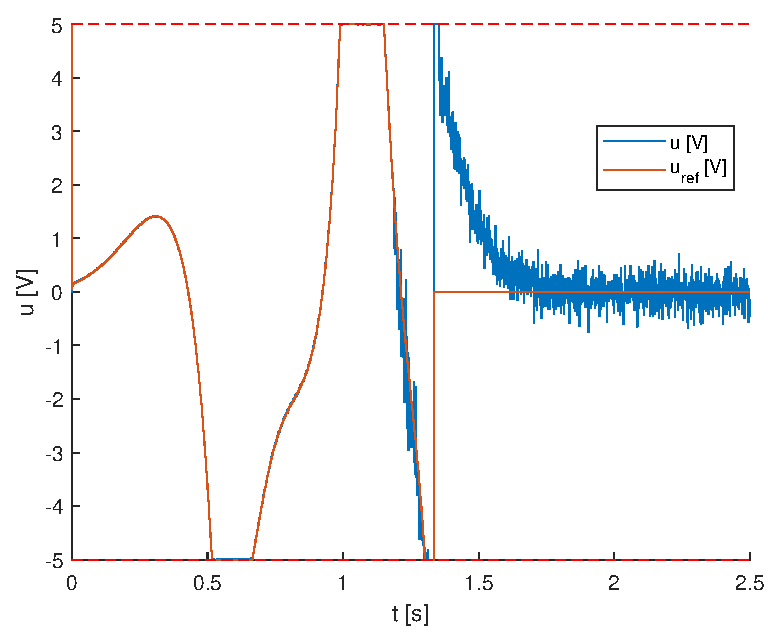
\includegraphics[width=0.6\linewidth]{slike/Control_EnergyShaping_trajectory.eps}
		\caption{Upravlja"cki signal generisan primenom \emph{energy shaping}}
		\label{fig:cntrl_energysh}
	\end{figure}
	
	\begin{figure}[!h]
		\centering
		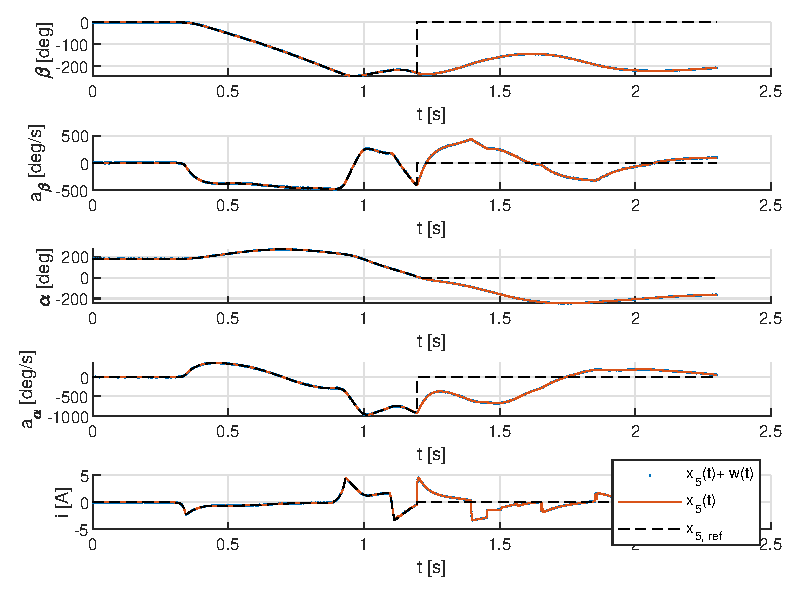
\includegraphics[width=.9\linewidth]{slike/States_EnergyShaping_trajectory.eps}
		\caption{Stanja sistema nakom primene upravljanja generisanog primenom \emph{energy shaping}}
		\label{fig:traj_energysh}
	\end{figure}
	\clearpage
	
	\begin{figure}[!h]
		\centering
		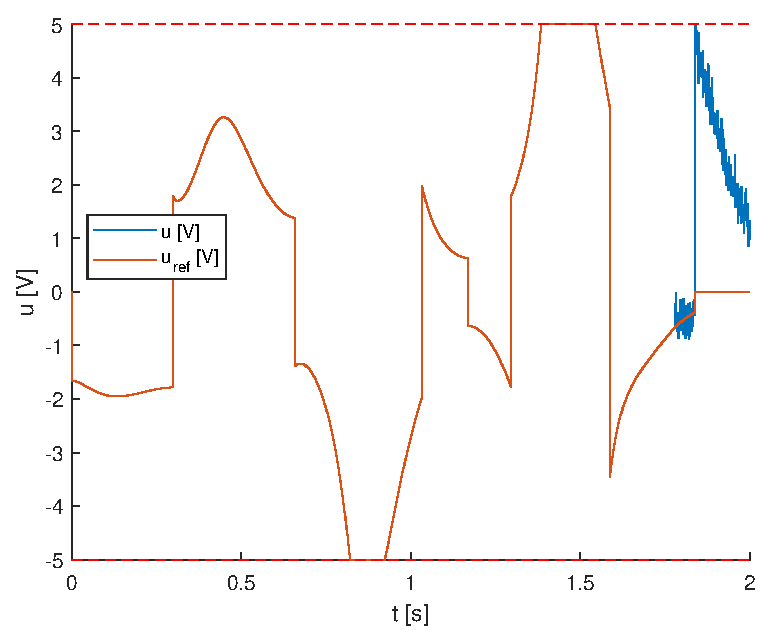
\includegraphics[width=0.6\linewidth]{slike/Control_ExpControl_trajectory.eps}
		\caption{Upravlja"cki signal generisan primenom \emph{exponentiation of the pendulum position}}
		\label{fig:cntrl_energyexp}
	\end{figure}
	
	\begin{figure}[!h]
		\centering
		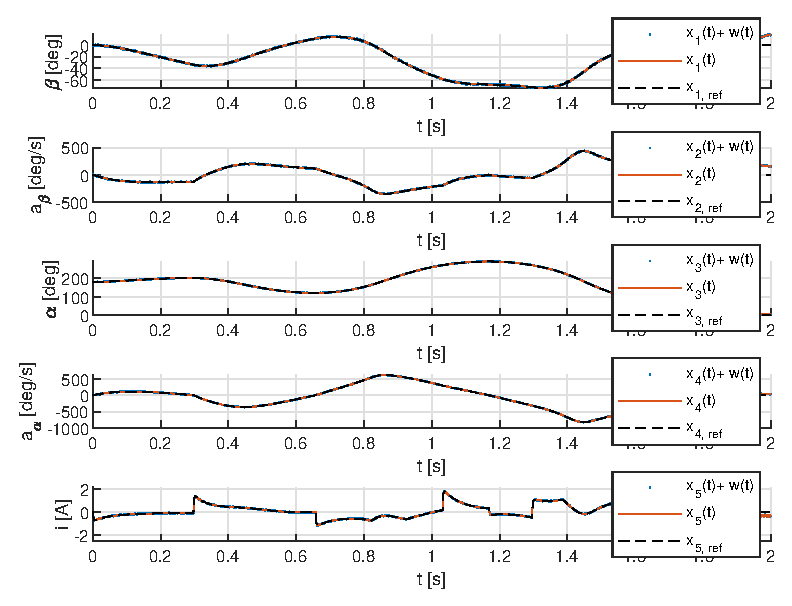
\includegraphics[width=.9\linewidth]{slike/States_ExpControl_trajectory.eps}
		\caption{Stanja sistema nakom primene upravljanja generisanog primenom \emph{exponentiation of the pendulum position}}
		\label{fig:traj_energyexp}
	\end{figure}
	\clearpage
	
	
	\subsubsection{Potiskivanje poreme\'caja u gornjem polo"zaju} \label{sec:por}
	
	\begin{figure}[!h]
		\centering
		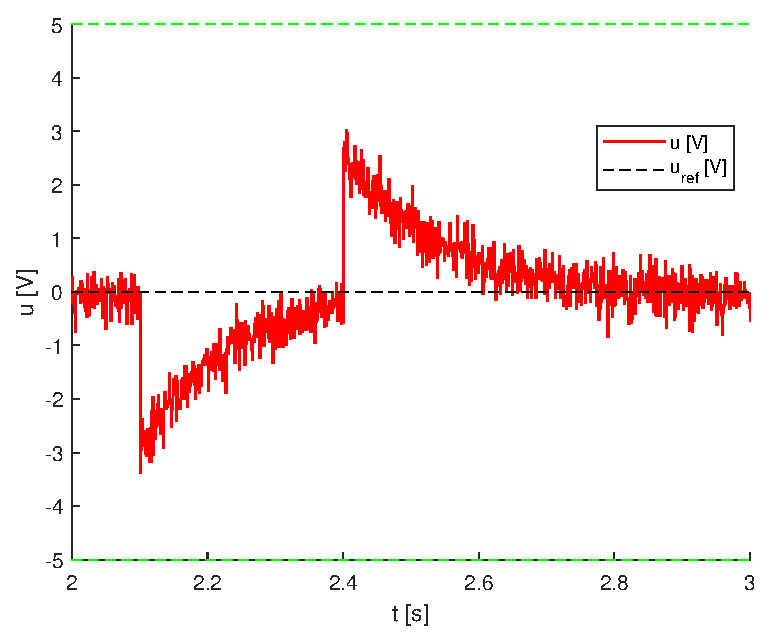
\includegraphics[width=0.52\linewidth]{slike/Control_dist.eps}
		\caption{Upravlja"cki tokom potiskivanja poreme\'caja}
		\label{fig:cnrl_dist}
	\end{figure}
	
	\begin{figure}[!h]
		\centering
		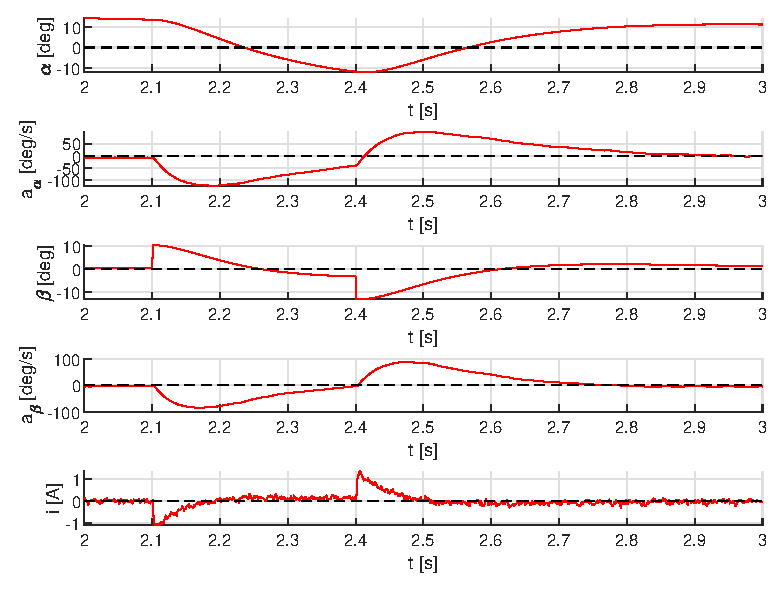
\includegraphics[width=.86\linewidth]{slike/States_dist.eps}
		\caption{Stanja sistema  tokom potiskivanja poreme\'caja}
		\label{fig:traj_dist}
	\end{figure}
	
	Projektovani LQR kontroler uspe"sno potiskuje poreme\'caj velike amplitude u uspravnom polo"zaju. Upravljanje je za"sumljeno zbog prisustva mernog "suma. Na osnovu slike (Slika \ref{fig:traj_dist}) mo"ze se primetiti da kontroler uspe"sno vrati sva stanja u koordinatni po"cetak osim ugla $\alpha$. Razlog za ovo pona"sanje je odsustvo uticaja ugla $\alpha$ na stabilnost u gornjem polo"zaju, odnosno ako nema potrebe menjati ugao $\beta$ ugao $\alpha$ mo"ze imati proizvoljnu vrednost.
	
	
	\clearpage
	\subsubsection{Tabelarni prikaz rezultata simulacije}\label{sec:tab}
	

	\begin{table}[!h]
		\begin{tabular}{lllllll}
			\cline{2-7}
			\multirow{2}{*}{} & \multicolumn{3}{c}{\emph{gain scheduling}} & \multicolumn{3}{c}{globalni LQR} \\ \cline{2-7} 
			& \multicolumn{1}{c}{$t_{16^o} [s]$} & \multicolumn{1}{c}{$t_s [s]$} & \multicolumn{1}{c}{$E_u [a.u.]$} & \multicolumn{1}{c}{$t_{16^o} [s]$} & \multicolumn{1}{c}{$t_s [s]$} & \multicolumn{1}{c}{$E_u [a.u.]$} \\ \hline
			MPC                
							 & 1.378      & 1.722      & 85.674      & 1.373   & 1.742  & \textbf{85.413}
							 \\ \hline
			\emph{energy control}
			                 &  1.539 & 1.600  & 185.306& 1.593   & 1.599  & 186.580
			                 \\ \hline
			\emph{exponentiation of the pendulum position}
			                 & 1.375  & 1.876  & 153.729& 1.381   & 1.928   & 156.399
			                 \\ \hline
			\emph{energy shaping}  
							 & 1.354  & 1.404  &126.975 & \textbf{1.355}   & \textbf{1.402}  & 127.173
			 				\\ \hline
		\end{tabular}
		\caption{Prikaz rezultata simulacije bez gre"ske modelovanja }
		\label{tab:no_error}
	\end{table}
	
	Na osnovu rezultata iz tabele \ref{tab:no_error} mo"zemo zaklju"citi slede\'ce: 
	\begin{itemize}
		\item Primena upravljanja na bazi MPC rezultuje najmanjim utro"skom energije.
		\item \emph{Energy control} je ujedno i najsporije i najskuplje upravljanje.
		\item \emph{Energy shaping} najbr"ze dosti"ze uspravni polo"zaj.
		\item Ako su gre"ske modelovanja zanemarljive globalni LQR i \emph{gain scheduling} su uporedivi.
	\end{itemize}
	\vspace{2cm}
	
	\begin{table}[!h]
		\begin{tabular}{lllllll}
			\cline{2-7}
			\multirow{2}{*}{} & \multicolumn{3}{c}{\emph{gain scheduling}} & \multicolumn{3}{c}{globalni LQR} \\ \cline{2-7} 
			& \multicolumn{1}{c}{$t_{16^o} [s]$} & \multicolumn{1}{c}{$t_s [s]$} & \multicolumn{1}{c}{$E_u [a.u.]$} & \multicolumn{1}{c}{$t_{16^o} [s]$} & \multicolumn{1}{c}{$t_s [s]$} & \multicolumn{1}{c}{$E_u [a.u.]$} \\ \hline
			MPC                
			& 1.373      & 1.708      & 85.341      & 1.376   & 1.736  & \textbf{84.989}
			\\ \hline
			\emph{energy control}
			&  1.542 & 1.602  & 185.669 & 1.54   & 1.598  & 186.333
			\\ \hline
			\emph{exponentiation of the pendulum position}
			& 1.374  & 1.868  & 153.365 & 1.380   & 1.932   & 155.301
			\\ \hline
			\emph{energy shaping}  
			& \textbf{1.356}  & \textbf{1.397}  &127.626 & 1.358   & 1.398  & 127.91
			\\ \hline
		\end{tabular}
		\caption{Prikaz rezultata simulacije sa gre"skom modelovanja }
		\label{tab:error}
	\end{table}
	
	Na osnovu rezultata iz tabele \ref{tab:error} mo"zemo zaklju"citi slede\'ce: 
	\begin{itemize}
		\item Primena upravljanja na bazi MPC rezultuje najmanjim utro"skom energije.
		\item \emph{Energy control} je ujedno i najsporije i najskuplje upravljanje.
		\item \emph{Energy shaping} najbr"ze dosti"ze uspravni polo"zaj.
		\item Ako su gre"ske modelovanja nisu zanemarljive bolje je primeniti \emph{gain scheduling}, u proseku je br"zi i tro"si manje energije.
	\end{itemize}
	
	
	\clearpage
	\section{Zaklju"cak}\label{sec:zakljucak}
	
	
	\newpage
	
	\begin{thebibliography}{9}
		\bibitem{inicijalna}
		\emph{Nonlinear control of an inverted pendulum}, António Samuel Ávila Balula, Thesis to obtain the Master of Science Degree in
		Engineering Physics 2016.
		
		\bibitem{energy_c}
		\emph{Swinging up the furuta pendulum and its stabi- ´
			lization via model predictive control.}, P. Seman, B. Rohal’-Ilkiv, M. Juhas, and M. Salaj.  Journal of Electrical Engineering, 64(3):152–158, 2013. ISSN
		13353632. doi: 10.2478/jee-2013-0022.
		\bibitem{ener_shaping}\emph{A normal form for energy shaping: application to the furuta pendulum}
		S. Nair and N. E. Leonard. 
		In Decision and Control, 2002, Proceedings of the 41st IEEE Conference on, volume 1, pages
		516–521. IEEE, 2002
		\bibitem{identifikacija}\emph{Identification of Dynamic System}, R. Isermann and M. Munchhof, Springer, 2011.
		
		\bibitem{mpc}\url{https://en.wikipedia.org/wiki/Model_predictive_control}
		\bibitem{rk4}\url{https://en.wikipedia.org/wiki/Runge%E2%80%93Kutta_methods}
		
		\bibitem{CASADI}\url{https://web.casadi.org/}
		
		\bibitem{multiple_shooting}\emph{Nonlinear Model Predictive Control Using Multiple Shooting Combined with 
		Collocation on Finite Elements}, Jasem Tamimi and Pu Li.
		
	\end{thebibliography}
\end{document}
